\documentclass{beamer}
\usepackage[utf8]{inputenc}
\usepackage{graphicx}
\usepackage[mode=buildnew]{standalone}
\usepackage{amsmath}
\usepackage{ragged2e}
\usepackage{tikz}
\usepackage{environ}
\usepackage{fontawesome}
\usepackage[justification=centering]{caption}
\usepackage{listings}
\usepackage{changepage}
\usepackage{bold-extra}
\usepackage{xcolor}
\usepackage{commath}
\usetikzlibrary{arrows,positioning,calc,decorations.pathreplacing, angles,quotes}
%\usepackage[most]{tcolorbox}
% \setbeamertemplate{footline}[frame number]
\graphicspath{{img/}}
\setbeamertemplate{navigation symbols}{}
\setbeamertemplate{page number in head/foot}{}
\setbeamertemplate{bibliography item}{}
\setbeamertemplate{caption}[numbered]
\setbeamercovered{transparent}
\renewcommand\refname{Bibliography}
\setbeamerfont{institute}{size=\small}
\usetheme{Frankfurt} % Of course!
\usecolortheme{whale}

\lstset{
  basicstyle=\small\ttfamily,
  columns=fullflexible,
  keepspaces=true,
  escapeinside={@@},
  keywordstyle=\bfseries,
  mathescape=true,
  morekeywords={not, show, sum, min, max, minimize, false},
  backgroundcolor=\color[gray]{0.95},
  rulecolor=\color{black},
  frame=single,
  framesep=7pt
}

\DeclareCaptionFormat{myformat}{\fontsize{5}{6}\selectfont#1#2#3}
\captionsetup{format=myformat}
\captionsetup[figure]{labelfont={bf},name={Fig.},labelsep=period}

\newcommand{\customframefont}[1]{
\setbeamertemplate{itemize/enumerate body begin}{#1}
\setbeamertemplate{itemize/enumerate subbody begin}{#1}
}

\NewEnviron{framefont}[1]{
\customframefont{#1} % for itemize/enumerate
{#1 % For the text outside itemize/enumerate
\BODY
}
\customframefont{\normalsize}
}

\setbeamertemplate{footline}{% 
  \hfill% 
  \usebeamercolor[fg]{page number in head/foot}% 
  \usebeamerfont{page number in head/foot}% 
  \insertframenumber%
  %\,/\,\inserttotalframenumber
  \kern1.2em\vskip4.5pt% 
}

\title{Elevator Project Report}
\subtitle{Target-Based Incremental Approach}
\author{Atreya Shankar, Luis Glaser \\[2pt] 
    \texttt{$\{$shankar,glaser$\}$@uni-potsdam.de}}
\institute{BM3: Advanced Problem Solving Techniques (ASP) \\ University of Potsdam, WiSe 2018/2019 \\ Prof. Dr. Torsten Schaub}
\date{April 8. 2019}

\begin{document}

\begin{frame}
\maketitle
\end{frame}

\begin{frame}
\frametitle{Table of Contents}
\setbeamertemplate{enumerate items}[square]
\begin{enumerate}
    \setlength\itemsep{1.5em}
    \item Introduction
    \item Target-Assignment Methodologies (Static)
    \item Translating Targets to Actions (Iterative)
    \item Optimizations
    \item Results
    \end{enumerate}
\end{frame}

\section{Introduction}
\subsection{}
\begin{frame}
\frametitle{Introduction}
\begin{columns}[T]
\begin{column}{.48\textwidth}
\vspace{-5pt}
\begin{figure}[hp]
    \centering
    \captionsetup{justification=centering}
    \setlength{\fboxsep}{0pt}
    \setlength{\fboxrule}{0.6pt}
    \fbox{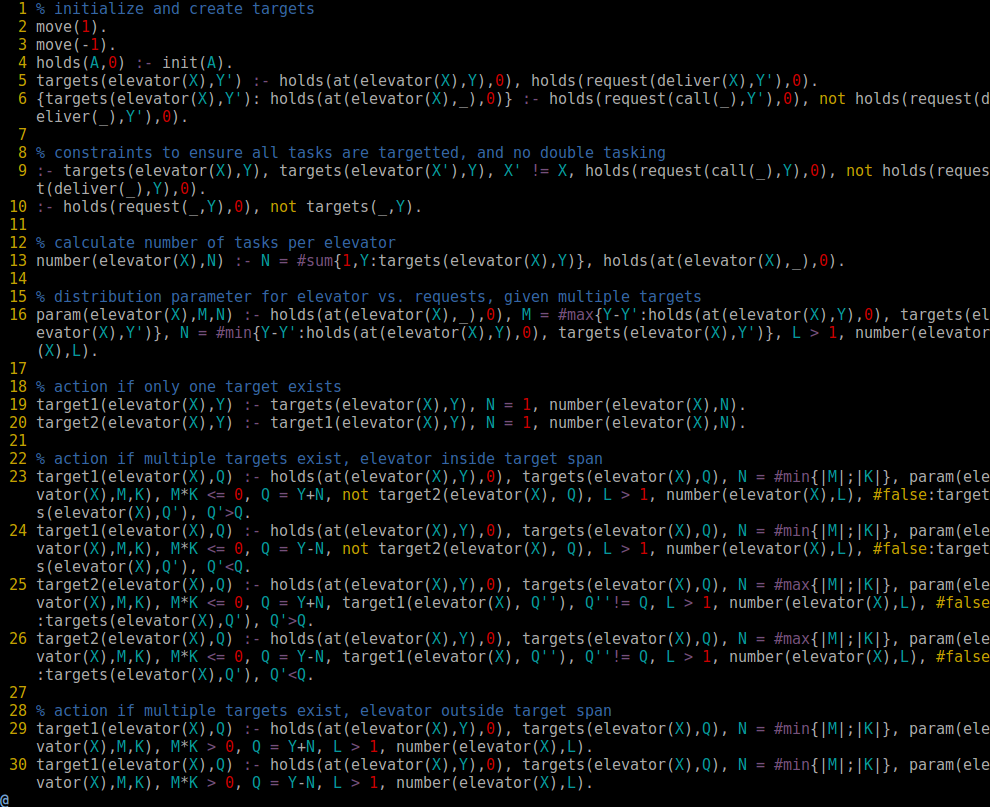
\includegraphics[width = 5cm]{source_code.png}}
    \caption{Snippet of encoding in elevator.lp}
    \label{fig1}
\end{figure}
\end{column}
\begin{column}{.55\textwidth}
\begin{itemize}
    \setlength\itemsep{2em}
    \item Encoding utilizes target-based incremental approach
    \item Approach deemed faster over a pure combinatorical approach
    \item Encoding succeeds on all Yeti cases
    \end{itemize}
\end{column}
\end{columns}
\end{frame}

\section{Target Assignment}
\subsection{}
\begin{frame}[fragile]
\frametitle{Target Assignment}
\begin{adjustwidth}{-1em}{-1em}
\begin{lstlisting}
@\textcolor{gray}{\slshape{$\%$ initialize and create targets}}@

targets(elevator(X),Y')
:- holds(at(elevator(X),Y),0), holds(request(deliver(X),Y'),0).

{targets(elevator(X),Y'): holds(at(elevator(X),_),0)}
:- holds(request(call(_),Y'),0), 
not holds(request(deliver(_),Y'),0).

@\textcolor{gray}{\slshape{$\%$ ensure no double targets and all requests targetted}}@

:- targets(elevator(X),Y), targets(elevator(X'),Y), X' != X, 
holds(request(call(_),Y),0), not holds(request(deliver(_),Y),0).

:- holds(request(_,Y),0), not targets(_,Y).
\end{lstlisting}
\end{adjustwidth}
\end{frame}

\subsection{}
\begin{frame}[fragile]
\frametitle{Distribution Parameter Generation}
\begin{adjustwidth}{-1em}{-1em}
\begin{lstlisting}
@\textcolor{gray}{\slshape{$\%$ calculate number of tasks per elevator}}@

number(elevator(X),N) :- N = #sum{1,Y:targets(elevator(X),Y)},
holds(at(elevator(X),_),0).

@\textcolor{gray}{\slshape{$\%$ distribution parameter given multiple targets}}@

param(elevator(X),M,N) :- holds(at(elevator(X),_),0), 
M = #max{Y-Y':holds(at(elevator(X),Y),0), 
targets(elevator(X),Y')}, 
N = #min{Y-Y':holds(at(elevator(X),Y),0), 
targets(elevator(X),Y')}, L > 1, number(elevator(X),L).
\end{lstlisting}
\begin{itemize}
    \setlength\itemsep{1em}
    \item Parameters are useful in deciphering position of elevator wrt. corresponding targets
\end{itemize}
\end{adjustwidth}
\end{frame}

\subsection{}
\begin{frame}
\frametitle{Target Distribution Cases I}
\begin{adjustwidth}{-1em}{-1em}
% make 4 possible cases here
\begin{figure}
\raggedright
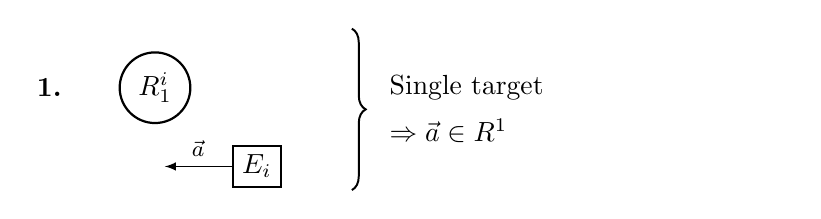
\begin{tikzpicture}[node distance=2cm,
req/.style={thick,circle,draw,font=\sffamily\normalsize},
ele/.style={thick,rectangle,draw,font=\sffamily\normalsize}]

\node[text width=3cm] at (0,0) {\bf1.};
\node[req] (1) {$R_{1}^i$};
\node[right=of 1] (2) {};
\node[ele, yshift=-1cm] (3) at ($(1)!0.5!(2)$) {$E_i$};
\node  at (3 -| 1) (E) {};
\draw [-latex] (3) -- node[above]{\footnotesize $\vec{a}$} (E);
\draw[line width=0.25mm,decoration={brace,amplitude=5pt,mirror},decorate]
(2.5,-1.3) -- node[text width=5cm, right=10pt] {Single target \\[5pt] $\Rightarrow \vec{a} \in \mathbb{R}^1$} (2.5,0.75);
\end{tikzpicture}\\
\vspace{30pt}

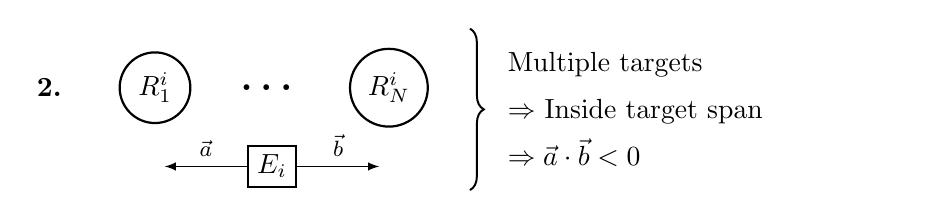
\begin{tikzpicture}[node distance=2cm,
req/.style={thick,circle,draw,font=\sffamily\normalsize},
ele/.style={thick,rectangle,draw,font=\sffamily\normalsize}]

\node[text width=3cm] at (0,0) {\bf2.};
\node[req] (1) {$R_{1}^i$};
\node[req, right=of 1] (2) {$R_{N}^i$};
\node[ele, yshift=-1cm] (3) at ($(1)!0.5!(2)$) {$E_i$};
\node  at (3 -| 1) (E) {};
\node  at (3 -| 2) (F) {};
\path (1) -- node[auto=false]{\bfseries\Large\ldots} (2);
\draw [-latex] (3) -- node[above]{\footnotesize $\vec{a}$} (E);
\draw [-latex] (3) -- node[above]{\footnotesize $\vec{b}$} (F);
\draw[line width=0.25mm,decoration={brace,amplitude=5pt,mirror},decorate]
(4,-1.3) -- node[text width=5cm, right=10pt] {Multiple targets \\[5pt] $\Rightarrow$ Inside target span \\[5pt] $\Rightarrow \vec{a}\cdot\vec{b} < 0$} (4,0.75);
\end{tikzpicture}\\
\end{figure}
\end{adjustwidth}
\end{frame}

\subsection{}
\begin{frame}
\frametitle{Target Distribution Cases II}
\begin{adjustwidth}{-1em}{-1em}
\begin{figure}
\raggedright
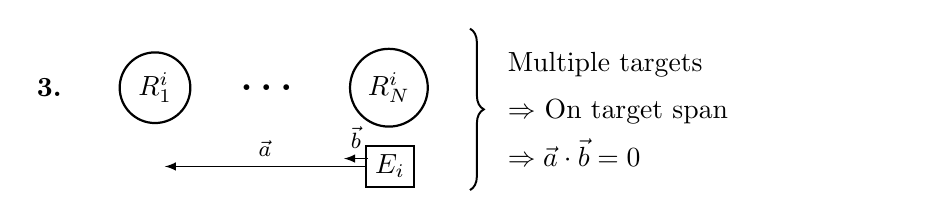
\begin{tikzpicture}[node distance=2cm,
req/.style={thick,circle,draw,font=\sffamily\normalsize},
ele/.style={thick,rectangle,draw,font=\sffamily\normalsize}]

\node[text width=3cm] at (0,0) {\bf3.};
\node[req] (1) {$R_{1}^i$};
\node[req, right=of 1] (2) {$R_{N}^i$};
\node[ele, yshift=-1cm,xshift = 1.5cm] (3) at ($(1)!0.5!(2)$) {$E_i$};
\node  at (3 -| 1) (E) {};
\path (1) -- node[auto=false]{\bfseries\Large\ldots} (2);
\draw [-latex] (3) -- node[above]{\footnotesize $\vec{a}$} (E);
\draw [-latex] (2.7,-0.9) -- node[above]{\footnotesize $\vec{b}$} (2.4,-0.9);
\draw[line width=0.25mm,decoration={brace,amplitude=5pt,mirror},decorate]
(4,-1.3) -- node[text width=5cm,right=10pt] {Multiple targets \\[5pt] $\Rightarrow$ On target span \\[5pt] $\Rightarrow \vec{a}\cdot\vec{b} = 0$} (4,0.75);
\end{tikzpicture}\\
\vspace{30pt}

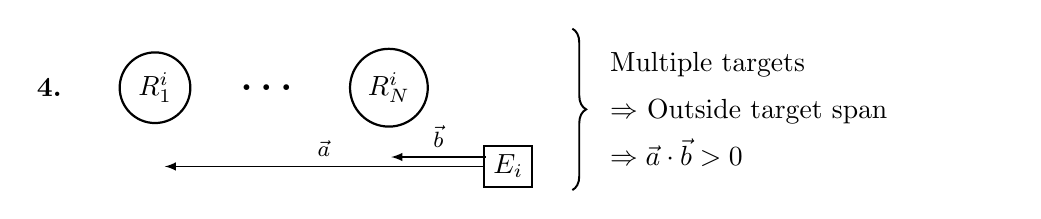
\begin{tikzpicture}[node distance=2cm,
req/.style={thick,circle,draw,font=\sffamily\normalsize},
ele/.style={thick,rectangle,draw,font=\sffamily\normalsize}]

\node[text width=3cm] at (0,0) {\bf4.};
\node[req] (1) {$R_{1}^i$};
\node[req, right=of 1] (2) {$R_{N}^i$};
\node[ele, yshift=-1cm, xshift = 3cm] (3) at ($(1)!0.5!(2)$) {$E_i$};
\node  at (3 -| 1) (E) {};
\node  at (3 -| 2) (F) {};
\path (1) -- node[auto=false]{\bfseries\Large\ldots} (2);
\draw [-latex] (3) -- node[above]{\footnotesize $\vec{a}$} (E);
\draw [-latex] (4.2,-0.88) -- node[above]{\footnotesize $\vec{b}$} (3,-0.88);
\draw[line width=0.25mm,decoration={brace,amplitude=5pt,mirror},decorate]
(5.3,-1.3) -- node[text width=5cm, right=10pt] {Multiple targets \\[5pt] $\Rightarrow$ Outside target span \\[5pt] $\Rightarrow \vec{a}\cdot\vec{b} > 0$} (5.3,0.75);
\end{tikzpicture}
\end{figure}
\end{adjustwidth}
\end{frame}

\subsection{}
\begin{frame}[fragile]
\frametitle{End-Targets Assignment I}
\begin{adjustwidth}{-1em}{-1em}
\textbf{Case 1 (Single Target):}
\vspace{5pt}
\begin{lstlisting}
target1(elevator(X),Y) :- targets(elevator(X),Y), N = 1, 
number(elevator(X),N).

target2(elevator(X),Y) :- target1(elevator(X),Y), N = 1, 
number(elevator(X),N).
\end{lstlisting}
\begin{itemize}
    \setlength\itemsep{1em}
    \item End-Targets are defined to be the same for consistency
    \item Necessary measure to keep end-targets framework
\end{itemize}
\end{adjustwidth}
\end{frame}

\subsection{}
\begin{frame}[fragile]
\frametitle{End-Targets Assignment II}
\begin{adjustwidth}{-1em}{-1em}
\textbf{Case 2/3 (Inside/On Span):}
\vspace{5pt}
\begin{lstlisting}[basicstyle=\scriptsize\ttfamily]
target1(elevator(X),Q) :- holds(at(elevator(X),Y),0), targets(elevator(X),Q), 
N = #min{|M|;|K|}, param(elevator(X),M,K), M*K <= 0, Q = Y+N, 
not target2(elevator(X), Q), L > 1, number(elevator(X),L), 
#false:targets(elevator(X),Q'), Q'>Q.

target1(elevator(X),Q) :- holds(at(elevator(X),Y),0), targets(elevator(X),Q), 
N = #min{|M|;|K|}, param(elevator(X),M,K), M*K <= 0, Q = Y-N, 
not target2(elevator(X), Q), L > 1, number(elevator(X),L), 
#false:targets(elevator(X),Q'), Q'<Q.

target2(elevator(X),Q) :- holds(at(elevator(X),Y),0), targets(elevator(X),Q), 
N = #max{|M|;|K|}, param(elevator(X),M,K), M*K <= 0, Q = Y+N, 
target1(elevator(X), Q''), Q''!= Q, L > 1, number(elevator(X),L), 
#false:targets(elevator(X),Q'), Q'>Q.

target2(elevator(X),Q) :- holds(at(elevator(X),Y),0), targets(elevator(X),Q), 
N = #max{|M|;|K|}, param(elevator(X),M,K), M*K <= 0, Q = Y-N, 
target1(elevator(X), Q''), Q''!= Q, L > 1, number(elevator(X),L), 
#false:targets(elevator(X),Q'), Q'<Q.
\end{lstlisting}
\end{adjustwidth}
\end{frame}

\subsection{}
\begin{frame}[fragile]
\frametitle{End-Targets Assignment III}
\begin{adjustwidth}{-1em}{-1em}
\textbf{Case 4 (Outside Span):}
\vspace{5pt}
\begin{lstlisting}[basicstyle=\scriptsize\ttfamily]
target1(elevator(X),Q) :- holds(at(elevator(X),Y),0), targets(elevator(X),Q), 
N = #min{|M|;|K|}, param(elevator(X),M,K), M*K > 0, Q = Y+N, L > 1,
number(elevator(X),L).

target1(elevator(X),Q) :- holds(at(elevator(X),Y),0), targets(elevator(X),Q), 
N = #min{|M|;|K|}, param(elevator(X),M,K), M*K > 0, Q = Y-N, L > 1,
number(elevator(X),L).

target2(elevator(X),Q) :- holds(at(elevator(X),Y),0), targets(elevator(X),Q), 
N = #max{|M|;|K|}, param(elevator(X),M,K), M*K > 0, Q = Y+N, 
target1(elevator(X), Q''), Q''!= Q, L > 1, number(elevator(X),L), 
#false:targets(elevator(X),Q'), Q'>Q.

target2(elevator(X),Q) :- holds(at(elevator(X),Y),0), targets(elevator(X),Q), 
N = #max{|M|;|K|}, param(elevator(X),M,K), M*K > 0, Q = Y-N,
target1(elevator(X), Q''), Q''!= Q, L > 1, number(elevator(X),L), 
#false:targets(elevator(X),Q'), Q'<Q.
\end{lstlisting}
\end{adjustwidth}
\end{frame}

\subsection{}
\begin{frame}[fragile]
\frametitle{Move Calculation}
\begin{adjustwidth}{-1em}{-1em}
\begin{lstlisting}
@\textcolor{gray}{\slshape{$\%$ calculate per-elevator moves}}@

moves(elevator(X),N) :- N = #sum{|Y-Y'|;|Y'-Y''|}, 
holds(at(elevator(X),Y),0), target1(elevator(X),Y'), 
target2(elevator(X),Y'').

@\textcolor{gray}{\slshape{$\%$ calculate cumulative moves}}@

allmoves(N) :- N = #sum{M:moves(elevator(_),M)}.
\end{lstlisting}
\begin{itemize}
    \setlength\itemsep{1em}
    \item Deterministic (pre-iterative) approach to quantify moves
    \item Useful for optimization/minimization purposes
\end{itemize}
\end{adjustwidth}
\end{frame}

\section{Target Actions}
\subsection{}
\begin{frame}[fragile]
\frametitle{Target Actions: Moving}
\begin{adjustwidth}{-1em}{-1em}
\begin{lstlisting}[basicstyle=\scriptsize\ttfamily]
@\textcolor{gray}{\slshape{$\%$ moving to target1}}@
do(elevator(X),move(V),t) :- holds(at(elevator(X),Y),t-1),
target1(elevator(X),Y'), holds(request(deliver(X),Y'),t), move(V),
|Y+V-Y'|<|Y-Y'|, not do(elevator(X),serve,t).

do(elevator(X),move(V),t) :- holds(at(elevator(X),Y),t-1), 
target1(elevator(X),Y'), holds(request(call(_),Y'),t), move(V),
|Y+V-Y'|<|Y-Y'|, not do(elevator(X),serve,t).

@\textcolor{gray}{\slshape{$\%$ moving to target2}}@
do(elevator(X),move(V),t) :- holds(at(elevator(X),Y),t-1), 
target2(elevator(X),Y'), holds(request(deliver(X),Y'),t), 
target1(elevator(X),Y''), move(V), |Y+V-Y'|<|Y-Y'|, 
not holds(request(deliver(X),Y''),t), not holds(request(call(_),Y''),t),
not do(elevator(X),serve,t).

do(elevator(X),move(V),t) :- holds(at(elevator(X),Y),t-1), 
target2(elevator(X),Y'), holds(request(call(_),Y'),t), 
target1(elevator(X),Y''),  move(V), |Y+V-Y'|<|Y-Y'|, 
not holds(request(deliver(X),Y''),t), not holds(request(call(_),Y''),t), 
not do(elevator(X),serve,t).
\end{lstlisting}
\end{adjustwidth}
\end{frame}

\subsection{}
\begin{frame}[fragile]
\frametitle{Target Actions: Serving}
\begin{adjustwidth}{-1em}{-1em}
\begin{lstlisting}
@\textcolor{gray}{\slshape{$\%$ serving delivery request}}@

do(elevator(X),serve,t) :- holds(request(deliver(X),Y),t-1), 
holds(at(elevator(X),Y),t-1), targets(elevator(X),Y).

@\textcolor{gray}{\slshape{$\%$ serving call request}}@

do(elevator(X),serve,t) :- holds(request(call(_),Y),t-1), 
holds(at(elevator(X),Y),t-1), targets(elevator(X),Y).

@\textcolor{gray}{\slshape{$\%$ serving floor}}@

serving(Y,t) :- do(elevator(X),serve,t), 
holds(at(elevator(X),Y),t-1).
\end{lstlisting}
\end{adjustwidth}
\end{frame}

\subsection{}
\begin{frame}[fragile]
\frametitle{Target Actions: Transfer Positions/Requests}
\begin{adjustwidth}{-1em}{-1em}
\begin{lstlisting}[basicstyle=\footnotesize\ttfamily]
@\textcolor{gray}{\slshape{$\%$ transfer elevator positions}}@

holds(at(elevator(X),Y+V),t) :- holds(at(elevator(X),Y),t-1), 
do(elevator(X),move(V),t).

holds(at(elevator(X),Y),t) :- holds(at(elevator(X),Y),t-1), 
do(elevator(X),serve,t).

holds(at(elevator(X),Y),t) :- holds(at(elevator(X),Y),t-1), 
not do(elevator(X),_,t).

@\textcolor{gray}{\slshape{$\%$ transfer requests}}@

holds(request(call(V),Y),t) :- holds(request(call(V),Y),t-1),
not serving(Y,t).

holds(request(deliver(X),Y),t) :- holds(request(deliver(X),Y),t-1), 
not holds(at(elevator(X),Y),t-1).
\end{lstlisting}
\end{adjustwidth}
\end{frame}

\section{Optimizations}
\subsection{}
\begin{frame}[fragile]
\frametitle{Optimizations}
\begin{adjustwidth}{-1em}{-1em}
% for optimizations, can talk about constraints to target choice rule, also for expansiveness allowing breaking up approach for evenly spaced distances
% optimizations: calculating total moves beforehand to minimize instead of doing it after
\begin{lstlisting}
@\textcolor{gray}{\slshape{$\%$ minimize deterministic cumulative moves}}@

#minimize{N:allmoves(N)}.
\end{lstlisting}
\begin{itemize}
    \setlength\itemsep{1em}
    \item Pre-iterative calculation of \texttt{allmoves(N)} makes minimization more efficient
    \item Reduction of target search-space in pre-solving phase
    \item Overall target assignment methodology more efficient than pure combinatorical approach
\end{itemize}
\end{adjustwidth}
\end{frame}

\section{Results}
\subsection{}
\begin{frame}[fragile]
\frametitle{Results}
\begin{columns}[T]
\begin{column}{.48\textwidth}
\vspace{-10pt}
\begin{figure}
    \centering
    \setlength{\fboxsep}{0pt}
    \fbox{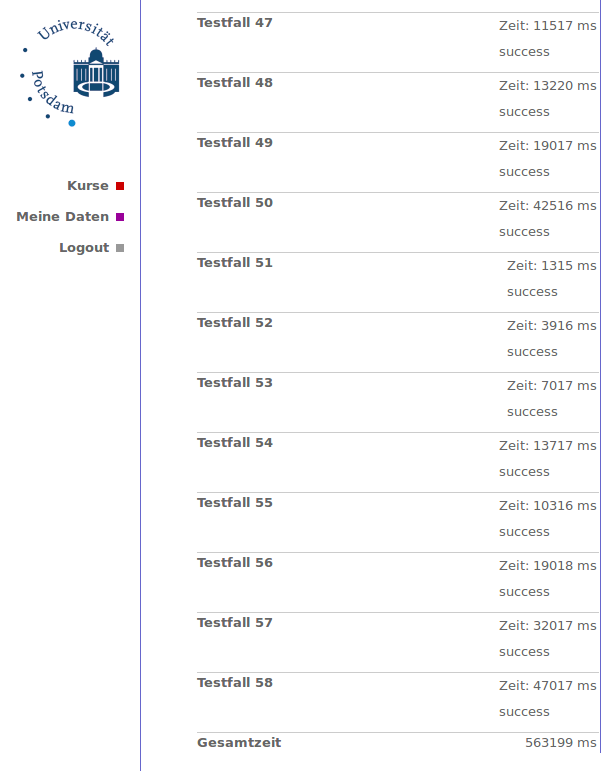
\includegraphics[width = 5cm]{yeti.png}}
    \caption{Snippet of Yeti performance for encoding}
    \label{fig2}
\end{figure}
\end{column}
\begin{column}{.52\textwidth}
\begin{itemize}
    \setlength\itemsep{1.5em}
    \item Encoding succeeds on all 58 Yeti test-cases
    \item Total runtime $\approx 560$s
    \item Longest runtime on ~~~~~~~~~~~instance 31 $\approx 85$s
    \item This was due to a large search space, resulting in 2048 optimal solutions
\end{itemize}
\end{column}
\end{columns}
\end{frame}

\end{document}